\chapter{Related Work}
In the ever expanding universe of information and the information overload that follows with it, the work on dealing with this overload never sleeps. This chapter will look at work done on handling information overload, especially considering news consumption, and news consumption on mobile devices. Topics like personalization, mobile news applications and news applications in general, designing mobile news applications and information aggregation will be discussed in more detail.

\section{Personalization on mobile devices}
Mobile Recommender Systems by Francesco Ricci



\section{Personalization regarding news apps}
User modeling for adaptive news access by Daniel Billsus and Michael J. Pazzani
\\\\
ePaper - the Personlized Mobile Newspaper by Shapira, Shoval, Meyer, Tractinsky, Mimran
\\\\
Aggregated Cross-Media News Visualization and Personalization by Cyril Rohr, Dian Tjondronegoro
\\\\
The Future of Personalization at News Websites - Lessons from a longitudinal study by Neil Thurman, Steve Schiffers

\subsection{Content Filtering}

\subsection{Collaborative Filtering	}

\section{News consumption}
How News Consumption is Shifting to the Personalized Social News Stream by Vadim Lavrusik

\section{UI Design mobile news applications}
News Sync: Three Reasons to Visualize News Better by V.G. Vinod .. .. .
\\\\
Designing the future of the newspaper by Anna Benckert van de Boel

\section{Commercial news recommendation applications}
There are a lot of different commercial news recommendation applications, and because of them being commercial, getting the information on how the applications solves information overload and personalization, can be quite tricky. Some of them have a rather good explanation on how it is done, but most of them keep their cards close to the chest.

Following are a short description of ten of the most popular and well known mobile news applications that are available at this time of writing, subjecting both the UI and how the recommendation is solved, if obtainable.


\subsection{Zite}
Zite is an intelligent magazine, which aims to guide the user towards discovering interesting things to read\cite{zite_appstore}, according to themselves.

\subsubsection{User Interface Design}
The Zite application meets the user with an infinite vertical scrollable view consisting of the top stories. Each news story is framed within a rectangular tile, whereas each tile consists of at least a title and the publisher of the article. The tile can also include tags, lead text, the time since it was published and the article's image (see the first image in figure \ref{screenshots_zite}).

From the top stories the user has several choices. In the top left corner the user can access his "quicklist" of categories and entities (see the last picture in figure \ref{screenshots_zite}). In the top right corner the user can search for topics like music or entities like Rolling Stones. These search results can be added to the "quicklist" to access them later. If an article is tapped, that article is showed in a new view (middle picture in figure \ref{screenshots_zite}). Here the user can read the Zite's version of the article or open the publisher's version. The user can share the article through numerous social websites and services. The article can be rated with thumbs up or thumbs down buttons. The user also has the ability to change the text size of the article or block the publisher of the article to never get another article from this publisher from this screen.

Zite has a clean and simple UI design with a minimum of surprises regarding navigation. All is more or less straight forward, with an exception of the swipe left on the main screen to trigger the next element on the "quicklist", which might come as a surprise to the common user.

\begin{figure}[!htbp]
\centering
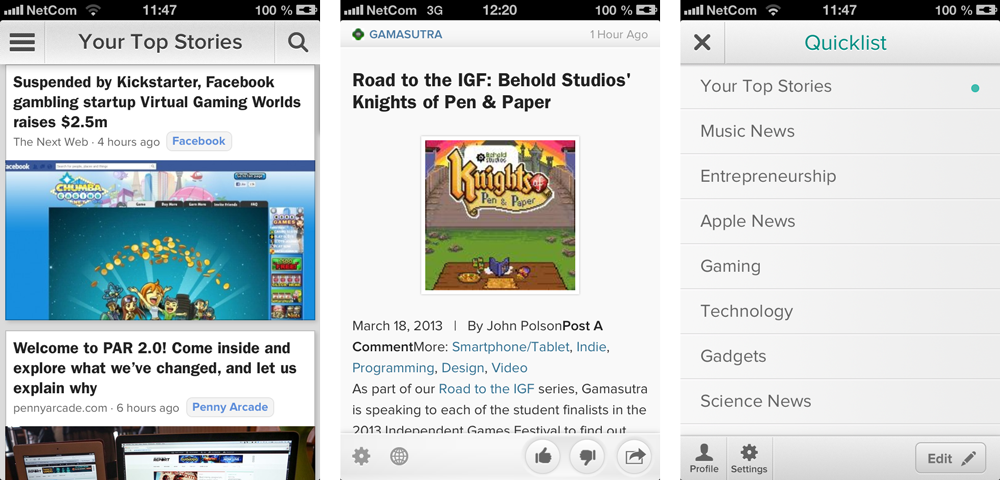
\includegraphics[width=130mm]{GFX/screenshots/zite.png}
\caption{Screenshots from Zite showing the Top Stories feed, a single news article, and categories list.}
\label{screenshots_zite}
\end{figure}

\subsubsection{Technology}
Zite uses different approaches to personalize the news magazine for the user\cite{zite_faq}. It uses automated algorithms to retrieve articles that are trending now by looking at how the different articles are discussed and shared on different websites, blogs, popular social network services, like Twitter and Facebook, and other news applications like Pocket and Google Reader. If an article is considered less trending by the algorithm, it is less likely to appear in the news stream, although the user might consider this article interesting.

The user can also choose to login with one or more of the aforementioned social network services and news applications, and get news recommendations based on what is shared by the user itself and friends of the user, or based on what is stored by the user in the news applications. 

Zite offers to save the user profile so the user can access its personalized news feed on different devices, but it does not limit the use of the application if a user chooses not to sign in.

The user can heavily influence what kind of news that are retrieved by rating different articles with the "thumbs up" or "thumbs down" buttons. The more rating the user gives, the better the personalization gets. Zite also keeps track of which articles the user is reading and which articles that are shared by the user and the user's connections on the social networks. This tracking influences the content delivered to the user.

In addition the user can search for different entities of interests, and further choose to like this type of entity by clicking a heart shaped button. If it is liked, this type of news will start to show in the main news stream. The user can also choose to add this entity to the "quicklist" to be able to quickly access only this type of news in the news stream.

A single source can also be blocked completely, as explained in the previous section.



\subsection{Flipboard}
Flipboard is a digital news magazine combining news of all sorts and events and feeds from social networks. Flipboard has gained much attention because of their joyful and easy-to-use flip-design.

\subsubsection{User Interface Design}
When launched, Flipboard greets the user with a front page consisting of different categories (see left image in figure \ref{screenshots_flipboard}). These categories are set by the user by clicking the "Your Flipboard" button shown in the right picture in figure \ref{screenshots_flipboard}. This settings screen is triggered by clicking the red ribbon in the top right corner of the start screen. While in the start screen the user can navigate further down by swiping or clicking one of the categories.

When a category is tapped, news articles from this category can be browsed by swiping up or down. Each category stream uses a full size view for each article, meaning that one article's preview uses the whole mobile screen. Each article's preview shows at least the title of the article, publisher and/or author, and the time since it was published. The preview can also include an image, lead text, and how many retweets\footnote{A retweet is if someone on Twitter shares a Twitter message created by someone else.} this article has. The user can also bring up the settings screen from this screen by tapping the magnifying glass in the top right corner.

When the article's preview is tapped, the user is presented with the article screen (see the middle picture in figure \ref{screenshots_flipboard}). Here the user can swipe up and down to read the whole story. If the article is retrieved from a social network, the user has the opportunity to interact with the social network the article is gathered from, like retweet and favorite for Twitter or "like" for Facebook. The user also has the ability to share the article via other services or choose to read it later by clicking the "out of the box" arrow on the top.

Flipboard has a joyous, pretty and easy to use interface design, and has gotten a lot of attention because the app is considered to have a beautiful design\cite{flipboard_design} and a special flip-like animation that is used when scrolling the pages.\cite{flipboard_video}\cite{flipboard_animation}. Flipboard was also picked as "App of the Year" by Apple in 2010\cite{flipboard_app_of_the_year}.

\begin{figure}[!htbp]
\centering
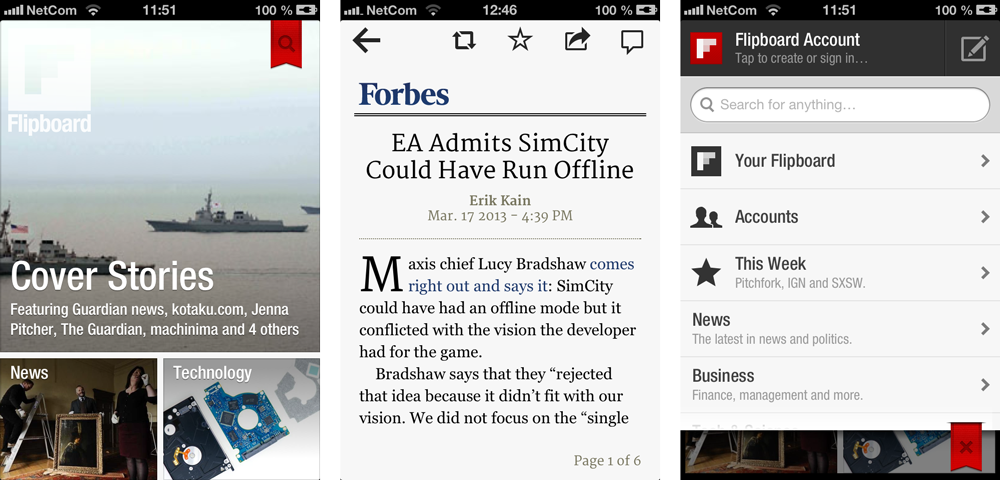
\includegraphics[width=130mm]{GFX/screenshots/flipboard.png}
\caption{Screenshots from Flipboard showing the top categories, a single news article, and the settings view.}
\label{screenshots_flipboard}
\end{figure}

\subsubsection{Technology}
Flipboard allows users to include their own social feeds from Twitter, Facebook, Google+, along with RSS feeds. Flipboard also crawls the Internet for trending news articles and categorizes them accordingly.

Flipboard acquired the Ellerdale startup early on\cite{flipboard_acquired_ellerdale}. The Ellerdale project included a semantic data-analysis technology which started as a Twitter trend analysis before it was acquired by Flipboard. Using Twitter's firehose API\footnote{The Twitter Firehose API allows third party developers to get access to all tweets that are composed in real-time.} the Ellerdale Project was able to process all tweets, thousands per second, and categorize them by topic, rather than keywords\cite{flipboard_categorize_by_topic} being able, in theory, to differentiate between Internet Explorer, Ford Explorer and Dora the Explorer. Further on Flipboard uses this technology to crawl social networks for trending topics and news, and being able to categorize them by topics to present useful and interesting news to the user.

The application offers the user the ability to create a Flipboard account to be able to access the personal feed on several devices. The application is still highly usable without creating an account, but some of the functionality is limited when not logged in. For instance, the user cannot save articles for later reading, like or comment articles without signing in.

\subsection{Pulse}

Pulse is a news reading application for iOS, Android and web browsers that supports HTML 5. It was released for the first time in 2010 and was awarded with the Apple Design Award of 2011\cite{pulse_apple_design_award}.

\subsubsection{User Interface Design}

When first booted, a login is required, either by a Pulse account or via Facebook. When logged in the first time, the user is presented with a limited set of news categories which the user can choose from to add to its interests. 

When done selecting category interests, the user is met with the main view, which is shown as the start up screen from now on, as shown in the first image in figure \ref{screenshots_pulse}. This screen shows one category with several publishers sorted in rows. By swiping horizontally in a publishers row, the user can browse the different articles from this publisher. By swiping vertically the user can browse the different publishers in this category. If the user swipes to the bottom of the screen, it can click the "Add Content" button, and add more sources of liking.

The sources can be removed by tapping the "Edit" button in the top right corner, and to change the displaying category, the user can hit the menu button in the top left corner. The user then has the ability to select another category (see the last image in figure \ref{screenshots_pulse}), or add more content to the news feeds.

The main screen has a lot of information showing at the same time and can feel somewhat cluttered and overloaded.

When an article is tapped, the single article screen is presented (see the middle image in figure \ref{screenshots_pulse}) to the user. This screen shows whatever information available from the source feed, like title, author, when the article was published, image and a lead text or article text if available. By hitting the action button in the top right corner, the user has the ability to save the article for later reading or sharing via Facebook, Twitter or email. 

By swiping horizontally the user can switch between the different articles from the showing publisher, similarly to the main screen. The user also has the ability to show the whole article by either tapping the title or pressing the "Read on Web" button at the bottom of the article. By doing so, the full article is presented in a web view, showing the publishers own website with the given article.

\begin{figure}[!htbp]
\centering
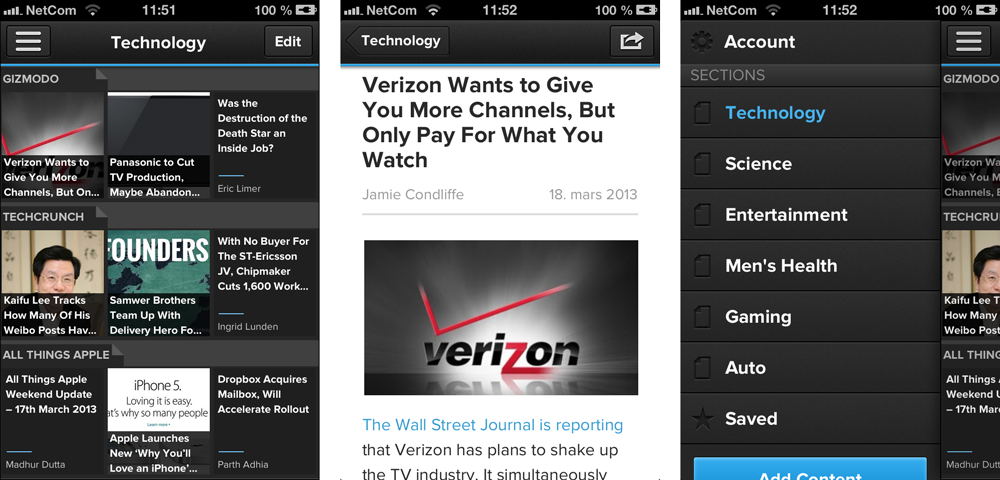
\includegraphics[width=130mm]{GFX/screenshots/pulse.png}
\caption{Screenshots from Pulse showing the start page, a single news article, and the categories/settings view.}
\label{screenshots_pulse}
\end{figure}

\subsubsection{Technology}

On first startup, after login, Pulse lets the user choose from a dozen or so different categories to start off the news reading experience. These different categories gets news from different predefined sources added by the developers. 

Pulse is mainly based on news publisher's RSS feeds, but allows the user to add their own social feeds from several social networking sites, e.g. Instagram, Facebook and YouTube.

The application also has the ability to search for feeds and add personal RSS feeds to a predefined category or a custom category. This way a user can add the newspaper feeds of their interests. Pulse can also check for the devices location and search for feeds that are nearby by using the GPS coordinates.

If logged in with Facebook, Pulse crawls the users news feed and finds articles previously shared or otherwise interacted with, and shows these article's sources in the recommended section.


\subsection{Summly}

Summly is a gesture oriented news aggregating application which was developed by Nick D'Aloisio in 2011. The main idea was not to personalize the news reading experience, but rather create intelligent summaries of the most trending news, by using advanced text analysis and natural language processing methods. Summly was sold to Yahoo for reported £18 million GBP in March 2013\cite{summly_sold_yahoo}, and was shortly after removed from the App Store, for Yahoo to use the summary technology elsewhere\cite{summly_closed}.

\subsubsection{User Interface Design}

\begin{figure}[!htbp]
\centering
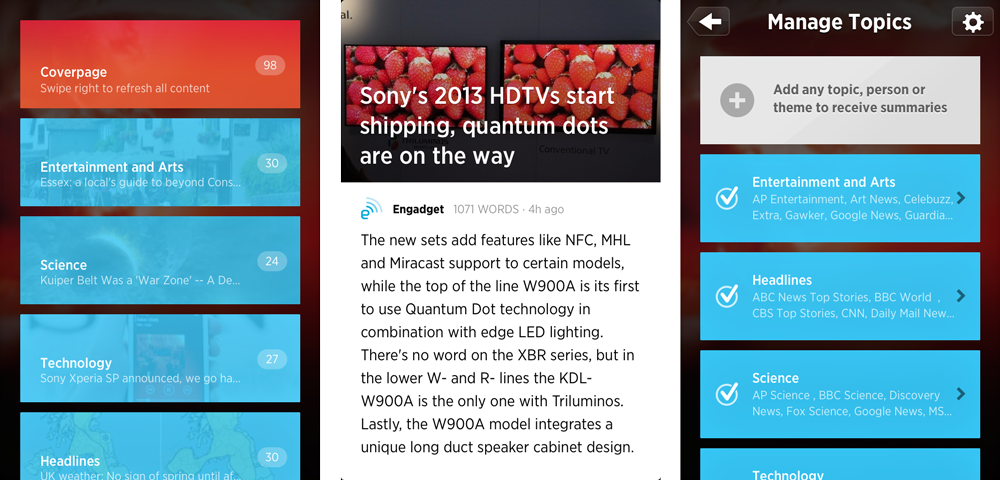
\includegraphics[width=130mm]{GFX/screenshots/summly.png}
\caption{Screenshots from Summly showing the category selection page, a single news article, and the category settings view.}
\label{screenshots_summly}
\end{figure}

\subsubsection{Technology}


\subsection{News360}

News360 is a news recommendation application and according to themselves a "smart and elegant app that learns what you like and brings you stories from across the web"\cite{news360_about}, available for iOS, Android and the Windows 8 series.

\subsubsection{User Interface Design}
On the first load, the user can choose to log in or continue without an account. Next, the user is prompted with a set of categories to select as interesting, a possibility to search for other entities to add to the feed, and an option to crawl the user's social news feeds for articles interacted with to add these topics to the personalization feed.

When the personal news feed is finished building, the home screen is presented to the user (see the first image in figure \ref{screenshots_news360}). This is also the first screen that meets the user when the application is launched after the initial setup is done the first time. News360 shows one news article per screen, and horizontal swiping is used to navigate to other stories. This screen shows the article image, if any, which category the story resides to, the title, publisher, how long ago since it was published and how many similar or related stories News360 has indexed.

By swiping down on this screen, the user can access the share screen, the "thumbs up" and "thumbs down" buttons to rate the article, and a save button, if the user wants to read the article later. By swiping up the user is presented with the lead text of the article and from here can choose to read the whole article by tapping the article or by hitting the "Continue" button.

When the single news article view is presented, the user has the same action buttons as by swiping down on the previous view, share, rate and save (see the second image in figure \ref{screenshots_news360} in the top right section.). In this view the user can choose to read more of the story, view the story from the publishers website, or choose a similar story by another publisher, to get the story from another angle or view. The user can also get more stories from this publisher by clicking the publisher's name. If the publishers name is tapped, the user can navigate to other stories by this publisher, see the publishers profile and choose to subscribe to this publisher.

By tapping the button in the top left corner in the main view (see first image in figure \ref{screenshots_news360}), the menu view is shown (see the last picture in figure \ref{screenshots_news360}). From here the user can navigate to the other categories or entities that it has added. The user can also get news by location, edit existing topics, add new topics, search for news, read saved stories, log in or out, and navigate to the settings section.


\begin{figure}[!htbp]
\centering
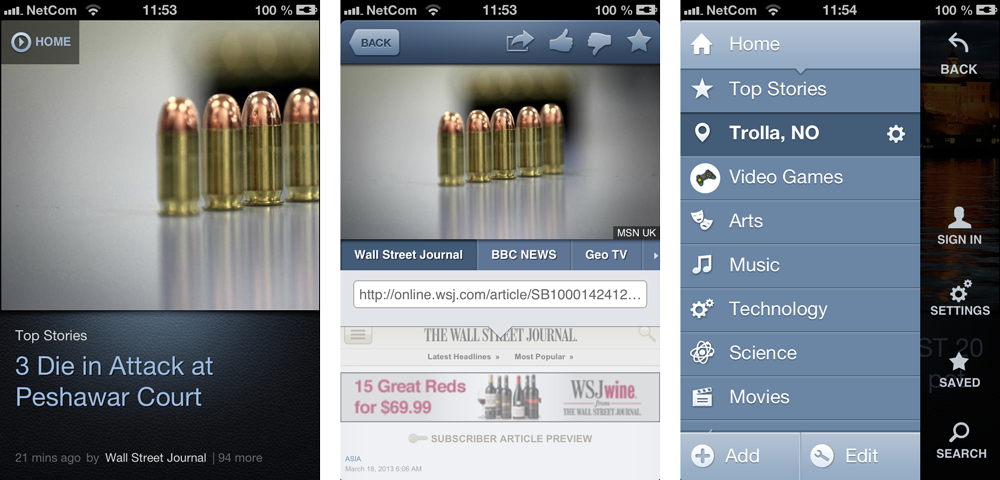
\includegraphics[width=130mm]{GFX/screenshots/news360.png}
\caption{Screenshots from News360 showing the top stories feed, a single news article, and the category settings/selection view.}
\label{screenshots_news360}
\end{figure}

\subsubsection{Technology}
News360 uses a lot of advanced technology to be able to recommend news to the reader\cite{news360_technology}. The semantic analysis platform is created from seven years of natural language analysis and development experience. News360 uses a self made sophisticated linguistic analysis engine to perform tasks like entity extraction, fact extraction, text classification, dossier generation and clusterization.

Further this engine is used in combination with a complex news-gathering system to analyze more than 100 000 articles a day in real time. From this analysis approximately 700 000 different people, locations, brands and companies are identified. Then the articles are tagged with locality and topics, and stored in clusters.

To understand which stories that are important, News360 uses a ranking algorithm which checks the impact of the sources that are aggregated, and all the articles that are published in that source. The system also checks the audience and credibility of the source and author, text characteristics and the velocity of the news event as it is happening.

News360 also gives the user the ability to tailor these recommended news by letting the application check the user's social feeds to find articles and sources interacted with. The user can rate each article with "thumbs up" or "thumbs down" buttons to have an impact on which news are shown.

With their semantic analysis, News360 also offers the user the ability to read similar stories, but from different publishers, to have the ability to view the news event from several points of view and angles.

A summary of the work flow, gathered from \cite{news360_technology}, is shown in figure \ref{tech_news360_workflow}.



\begin{figure}[!htbp]
\centering
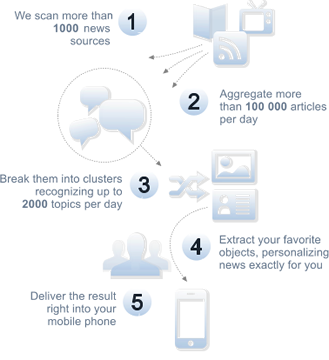
\includegraphics[width=70mm]{GFX/tech/news360workflow.png}
\caption{The workflow of the News360 news system}
\label{tech_news360_workflow}
\end{figure}


\subsection{Circa}

\subsubsection{User Interface Design}

\begin{figure}[!htbp]
\centering
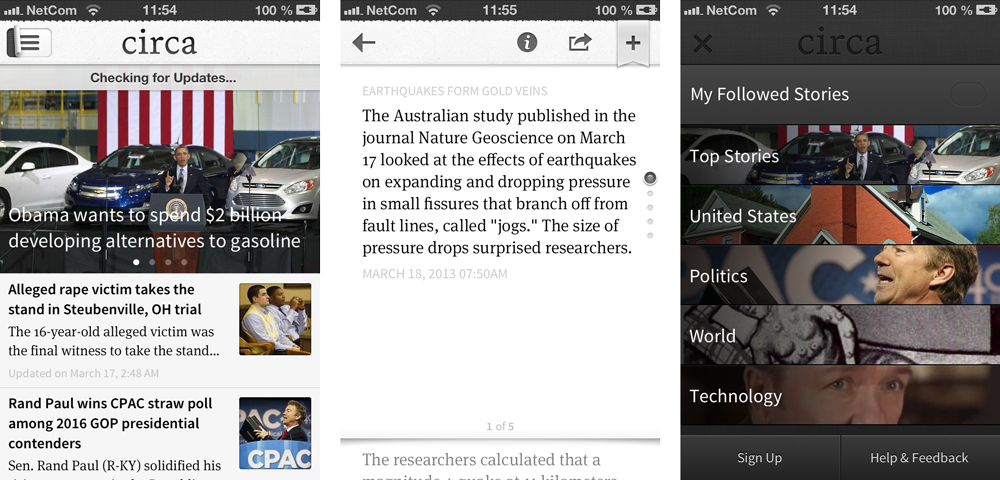
\includegraphics[width=130mm]{GFX/screenshots/circa.png}
\caption{Screenshots from Circa showing the top stories feed, a single news article, and the category selection view.}
\label{screenshots_circa}
\end{figure}

\subsubsection{Technology}


\subsection{Wavii}

\subsubsection{User Interface Design}

\begin{figure}[!htbp]
\centering
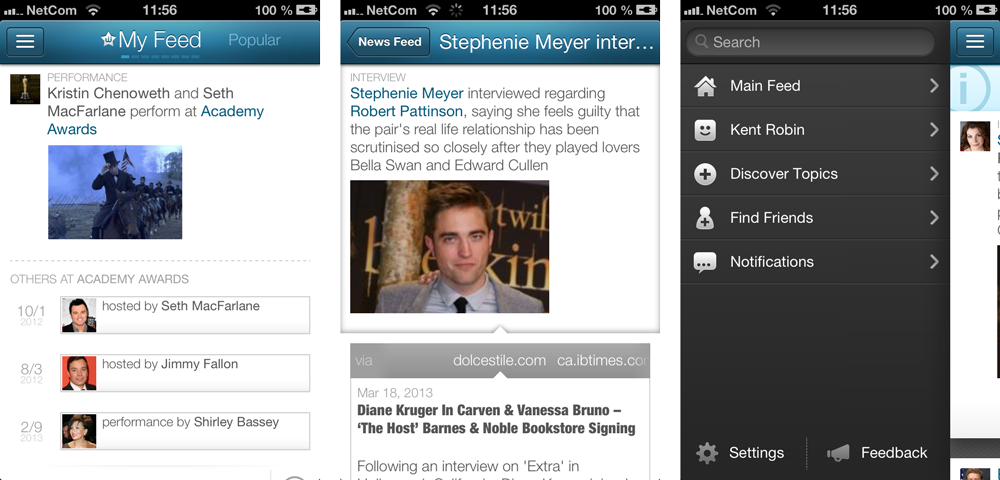
\includegraphics[width=130mm]{GFX/screenshots/wavii.png}
\caption{Screenshots from Wavii showing the top stories feed, a single news article, and the category selection/settings view.}
\label{screenshots_wavii}
\end{figure}

\subsubsection{Technology}


\subsection{Prismatic}

\subsubsection{User Interface Design}

\begin{figure}[!htbp]
\centering
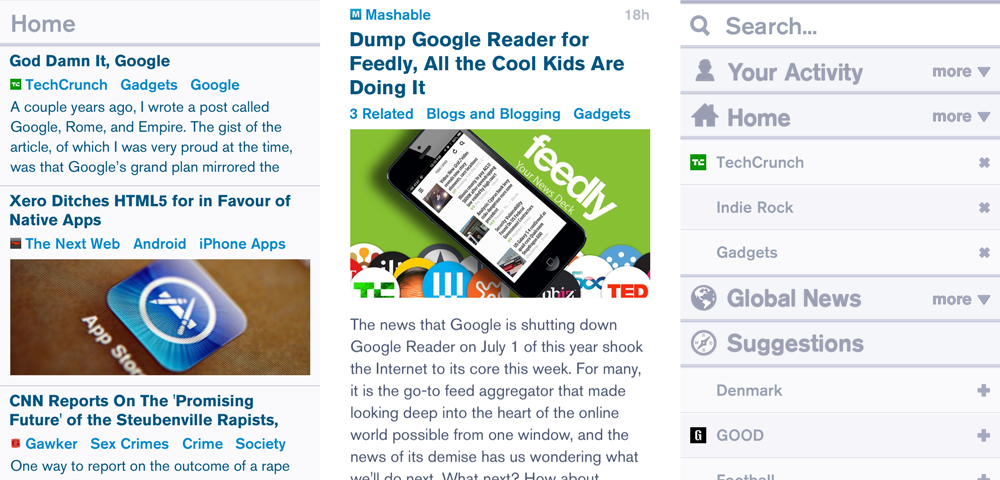
\includegraphics[width=130mm]{GFX/screenshots/prismatic.png}
\caption{Screenshots from Prismatic showing the top stories feed, a single news article, and the category selection/settings view.}
\label{screenshots_prismatic}
\end{figure}

\subsubsection{Technology}


\subsection{Taptu}

\subsubsection{User Interface Design}

\begin{figure}[!htbp]
\centering
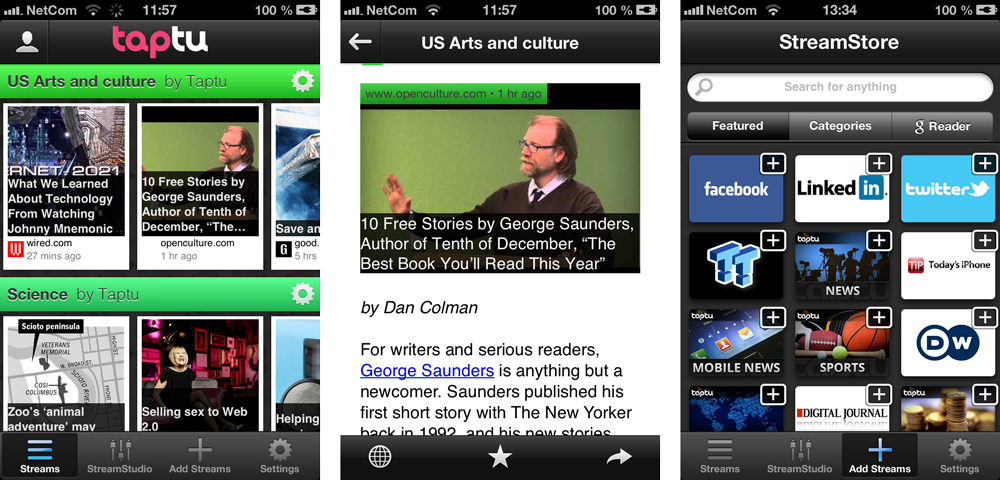
\includegraphics[width=130mm]{GFX/screenshots/taptu.png}
\caption{Screenshots from Taptu showing the top stories feed, a single news article, and the category settings view.}
\label{screenshots_taptu}
\end{figure}

\subsubsection{Technology}


\subsection{Feedly}

\subsubsection{User Interface Design}

\begin{figure}[!htbp]
\centering
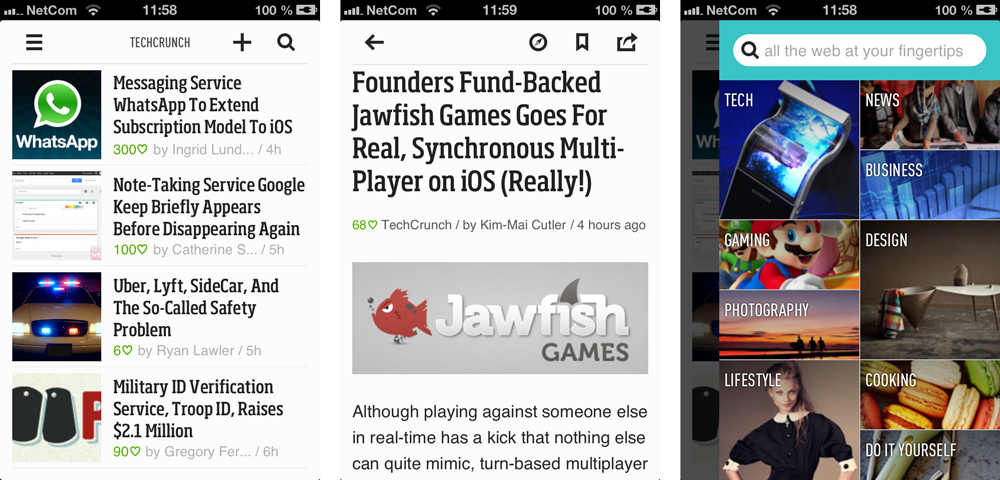
\includegraphics[width=130mm]{GFX/screenshots/feedly.png}
\caption{Screenshots from Feedly showing the top stories feed, a single news article, and the category settings view.}
\label{screenshots_feedly}
\end{figure}

\subsubsection{Technology}


\subsection{Comparing the Commercial Applications}

\begin{center}
    \begin{tabular}{ | l | l | l | l | l | l | l | l | l | l | l |}
    \hline
    Feature/Apps & Zite & Flipboard & Pulse & Summly & News360 & Circa & Wavii & Prismatic & Taptu & Feedly \\ \hline
     
    News Sources & N/A & N/A & N/A & N/A & N/A & N/A & N/A & N/A & N/A & N/A  \\ \hline
     
    Clear/Cluttered UI & N/A & N/A & N/A & N/A & N/A & N/A & N/A & N/A & N/A & N/A  \\ \hline
     
    Filtering & N/A & N/A & N/A & N/A & N/A & N/A & N/A & N/A & N/A & N/A  \\ \hline

    Sharing & N/A & N/A & N/A & N/A & N/A & N/A & N/A & N/A & N/A & N/A  \\ \hline

    Login & N/A & N/A & N/A & N/A & N/A & N/A & N/A & N/A & N/A & N/A  \\ \hline
    \end{tabular}
\end{center}

